% CHI Extended Abstracts template.% THIS IS SIGPROC-SP.TEX - VERSION 3.1
% WORKS WITH V3.2SP OF ACM_PROC_ARTICLE-SP.CLS
% APRIL 2009
%
% It is an example file showing how to use the 'acm_proc_article-sp.cls' V3.2SP
% LaTeX2e document class file for Conference Proceedings submissions.
% ----------------------------------------------------------------------------------------------------------------
% This .tex file (and associated .cls V3.2SP) *DOES NOT* produce:
%       1) The Permission Statement
%       2) The Conference (location) Info information
%       3) The Copyright Line with ACM data
%       4) Page numbering
% ---------------------------------------------------------------------------------------------------------------
% It is an example which *does* use the .bib file (from which the .bbl file
% is produced).
% REMEMBER HOWEVER: After having produced the .bbl file,
% and prior to final submission,
% you need to 'insert'  your .bbl file into your source .tex file so as to provide
% ONE 'self-contained' source file.
%
% Questions regarding SIGS should be sent to
% Adrienne Griscti ---> griscti@acm.org
%
% Questions/suggestions regarding the guidelines, .tex and .cls files, etc. to
% Gerald Murray ---> murray@hq.acm.org
%
% For tracking purposes - this is V3.1SP - APRIL 2009

\documentclass{acm_proc_article-sp}

\begin{document}

\title{Towards electronic digital music practice for neurodiverse people}
% \title{A Sample {\ttlit ACM} SIG Proceedings Paper in LaTeX Format\titlenote{(Does NOT produce the permission block, copyright information nor page numbering). For use with ACM\_PROC\_ARTICLE-SP.CLS. Supported by ACM.}}
% \subtitle{[Extended Abstract]
% \titlenote{}
%
% You need the command \numberofauthors to handle the 'placement
% and alignment' of the authors beneath the title.
%
% For aesthetic reasons, we recommend 'three authors at a time'
% i.e. three 'name/affiliation blocks' be placed beneath the title.
%
% NOTE: You are NOT restricted in how many 'rows' of
% "name/affiliations" may appear. We just ask that you restrict
% the number of 'columns' to three.
%
% Because of the available 'opening page real-estate'
% we ask you to refrain from putting more than six authors
% (two rows with three columns) beneath the article title.
% More than six makes the first-page appear very cluttered indeed.
%
% Use the \alignauthor commands to handle the names
% and affiliations for an 'aesthetic maximum' of six authors.
% Add names, affiliations, addresses for
% the seventh etc. author(s) as the argument for the
% \additionalauthors command.
% These 'additional authors' will be output/set for you
% without further effort on your part as the last section in
% the body of your article BEFORE References or any Appendices.

\numberofauthors{6} %  in this sample file, there are a *total*
% of EIGHT authors. SIX appear on the 'first-page' (for formatting
% reasons) and the remaining two appear in the \additionalauthors section.
%
\author{
% You can go ahead and credit any number of authors here,
% e.g. one 'row of three' or two rows (consisting of one row of three
% and a second row of one, two or three).
%
% The command \alignauthor (no curly braces needed) should
% precede each author name, affiliation/snail-mail address and
% e-mail address. Additionally, tag each line of
% affiliation/address with \affaddr, and tag the
% e-mail address with \email.
%
% 1st. author
\alignauthor
Till Bovermann\\
       \affaddr{Department of Media}\\
       \affaddr{Aalto University}\\
       \affaddr{Helsinki}\\
       \email{till.bovermann@aalto.fi}
% 2nd. author
\alignauthor
Julian Parker\\
       \affaddr{Department of Signal Processing and Acoustics}\\
       \affaddr{Aalto University}\\
       \affaddr{Helsinki}\\
       \email{julian.parker@aalto.fi}
% 3rd. author
\alignauthor Ramyah Gowrishankar\\
       \affaddr{Department of Design}\\
       \affaddr{Aalto University}\\
       \affaddr{Helsinki}\\
       \email{ramyah.gowrishankar@aalto.fi}
\and  % use '\and' if you need 'another row' of author names
% 4th. author
\alignauthor Mila Moisio\\
       \affaddr{TAUKO}\\
       \affaddr{Helsinki}\\
       % \affaddr{}\\
       \email{mila@taukovaatteet.com}
% 5th. author
\alignauthor  Jussi Mikkonen\\
       \affaddr{Department of Design}\\
       \affaddr{Moffett Field}\\
       \affaddr{California 94035}\\
       \email{fogartys@amesres.org}
% 6th. author
\alignauthor Charles Palmer\\
       \affaddr{Palmer Research Laboratories}\\
       \affaddr{8600 Datapoint Drive}\\
       \affaddr{San Antonio, Texas 78229}\\
       \email{cpalmer@prl.com}
}
% There's nothing stopping you putting the seventh, eighth, etc.
% author on the opening page (as the 'third row') but we ask,
% for aesthetic reasons that you place these 'additional authors'
% in the \additional authors block, viz.
\date{02.05.2013}
% Just remember to make sure that the TOTAL number of authors
% is the number that will appear on the first page PLUS the
% number that will appear in the \additionalauthors section.

\maketitle
\begin{abstract}
	This paper gives an overview on the DEIND project which aims to connect neurodiverse people with the field of contemporary electronic and digital music practice. 
	In pursuit of this, people with autistic spectrum disorders are invited to take part in the design process of electronic instruments.

	To facilitate music practice, we aim for a holistic instrument experience rather than a modular approach in which the underlying modules of electronic instruments may become too evident and possibly confuse the player too much.

	The close integration of target group members encourages a bilateral learning process: on the one hand, there is an intense and fruitful experience for the participants developing, on the other hand, involved researchers will identify design challenges specific to the target group yet very likely reveal new perspectives on the broader view of their respective area of research.
\end{abstract}

% TODO add categories terms and keywords
% % A category with the (minimum) three required fields
% \category{H.4}{Information Systems Applications}{Miscellaneous}
% %A category including the fourth, optional field follows...
% \category{D.2.8}{Software Engineering}{Metrics}[complexity measures, performance measures]

% \terms{Theory}

% \keywords{ACM proceedings, \LaTeX, text tagging} % NOT required for Proceedings

\section{Introduction}


%ACKNOWLEDGMENTS are optional
\section{Acknowledgments}
This research was part of the DEIND project on designing electronic instruments for neurodiverse people, funded by the Aalto Media Factory of Aalto University, Helsinki.  

\bibliographystyle{abbrv}
\bibliography{sigproc} 
\balancecolumns
% That's all folks!
\end{document}

% Tested with XeTeX on Mac OS X (Get it from http://tug.org/mactex)
% The latest version is available at <http://manas.tungare.name/software/latex/>
% 
% Filename: chi-ext.cls
% 
% CHANGELOG:
%   2010-10-18   Manas Tungare      Restored support for \figures.
%   2010-08-09   Manas Tungare      Updated copyright info for CHI 2011
%   2009-12-04   Stephen Voida      Updated copyright info for CHI 2010
%   2008-11-25   Manas Tungare      Initial create.
%   2009-11-17   Manas Tungare      Refactored the title & author sections.
% 
% LICENSE:
%   Public domain: You are free to do whatever you want with this template.
%   If you improve this in any way, please drop me a note <manas@tungare.name>,
%   so I can share the updates with everyone.
%   
%   PLEASE RECONSIDER BEFORE FORKING THIS TEMPLATE; there are already
%   several versions of the chiproceedings template for no good reason.
%   DO NOT REDISTRIBUTE THIS FILE UNDER A DIFFERENT FILENAME unless you
%   have a very good reason to change its name.

\documentclass{chi-ext}

\title{Electronic digital music practice for\newline neurodiverse people: a work in progress}

\author{
  \textbf{Till Bovermanṇ} \\
  AuthorCo, Inc. \\
  123 Author Ave. \\
  Authortown, PA 54321 USA \\
  author1@anotherco.com \\
  \\
  \textbf{Julian Parker} \\
  VP, Authoring \\
  Authorship Holdings, Ltd. \\
  Authors Square \\
  Authorfordshire, UK AU1 2JD \\
  author2@author.ac.uk \\
  \\
  \textbf{Third Author} \\
  AnotherCo, Inc. \\
  123 Another Ave. \\
  Anothertown, PA 54321 USA \\
  author3@anotherco.com \\
  % \\
  % \textbf{Till Bovermanṇ} \\
  % AuthorCo, Inc. \\
  % 123 Author Ave. \\
  % Authortown, PA 54321 USA \\
  % author1@anotherco.com \\
  % \\
  % \textbf{Second Author} \\
  % VP, Authoring \\
  % Authorship Holdings, Ltd. \\
  % Authors Square \\
  % Authorfordshire, UK AU1 2JD \\
  % author2@author.ac.uk \\
  % \\
  % \textbf{Third Author} \\
  % AnotherCo, Inc. \\
  % 123 Another Ave. \\
  % Anothertown, PA 54321 USA \\
  % author3@anotherco.com \\
}

\keywords{Keywords go here.}

\acmclassification{H.5.2 Information Interfaces and Presentation: User interfaces –
Evaluation/ methodology}

\copyrightinfo{
  Copyright is held by the author/owner(s). \\
  \emph{CHI 2011}, May 7--12, 2011, Vancouver, BC, Canada. \\
  ACM  978-1-4503-0268-5/11/05. \\
}

% Repeat author names (minus affiliations and addresses) and title here 
% for PDF metadata.
\hypersetup{
  pdfauthor={Till Bovermann, Julian Parker, Third Author},
  pdfkeywords={Keyword 1, Keyword 2},
  pdfsubject={General Subject Area},
  pdftitle={Electronic music practice for neurodiverse people -- a work in progress},
}

\begin{document}
\maketitle

\begin{multicols}{2}
  
\makeauthors
\makecopyright

\section{Abstract}
This paper gives an overview of the DEIND project. DEIND is an attempt to connect neurodiverse people with the field of contemporary electronic and digital music practice. 

In pursuit of this, people with autistic spectrum disorders are invited to take part in the design process of electronic instruments.
% To facilitate music practice, we aim for a holistic instrument experience rather than a modular approach in which the underlying modules of electronic instruments may become too evident and possibly confuse the player too much.

The close integration of target group members into the research process encourages a bilateral learning process: on the one hand, there is an intense and fruitful experience for the participants. On the other hand, involved researchers can identify design challenges specific to the target group and reveal new perspectives on their respective area of research.

\section{Keywords}
\makeatletter \@keywords \makeatother

\section{ACM Classification Keywords}
\makeatletter \@acmclassification \makeatother

%--------------------------------------------------------------
% \columnbreak

\section{Motivation}

As a consequence of recent technological and cultural developments -- cheap electronics, rapid prototyping technologies, freely available information -- the majority of people in the western world are able to express themselves creatively with technology in a multitude of ways without the large investment of time or money that would have been traditionally necessary. 
This has manifested itself in the birth of the DIY, maker and demo scenes.

%Apart from mainstream hypes such as the hipstamatic phenomenon\footnote{See e.g. \url{http://www.kunsthal.nl/%en-22-681-Hipstamatic.html}} the tools for digital content creation as well established social and cultural niches %featuring unique expression vocabularies, e.g., embodied by experimental electronic music practice.

People with disabilities however, often lack the possibility to take part in such cutting-edge movements.\footnote{Although freedom of artistic expression is seen as a human right \cite{shaheed2013-rep}.} 
This is because the necessary assistive features and design considerations are often of secondary interest to the designers and developers of the required technology. 
This problem is exacerbated further when it comes to the facilitation of participation in cultural niches\footnote{This is not due to bad faith on the part of the designers, but merely lack of information or resources.}.

However, questions remain on how, for example, electronic music practice (\emph{EMP}) can be scaffolded to support people facing challenges in society due to differences in their neurologic development:
How can \emph{EMP} support them in expressing themselves beyond the mainstream? 
How can it make the engaging nature of \emph{EMP} accessible for them without providing too much guidance?
Can \emph{EMP} empower them to shape their own social niche(s) in the above-mentioned sense?

This paper gives an overview on how the DEIND project, which aims to connect neurodiverse (\emph{ND}) people with the field of contemporary electronic and digital music practice, approaches these questions.
In pursuit of this, people with autistic spectrum disorders are invited to participate in the design process of electronic musical instruments. 
To facilitate music practice, we aim for a holistic instrument experience rather than a modular approach in which the underlying modules of electronic instruments, interface \& mapping \& sound synthesis, would become too evident and possibly interfere with the flow experience. 

\begin{figure}
	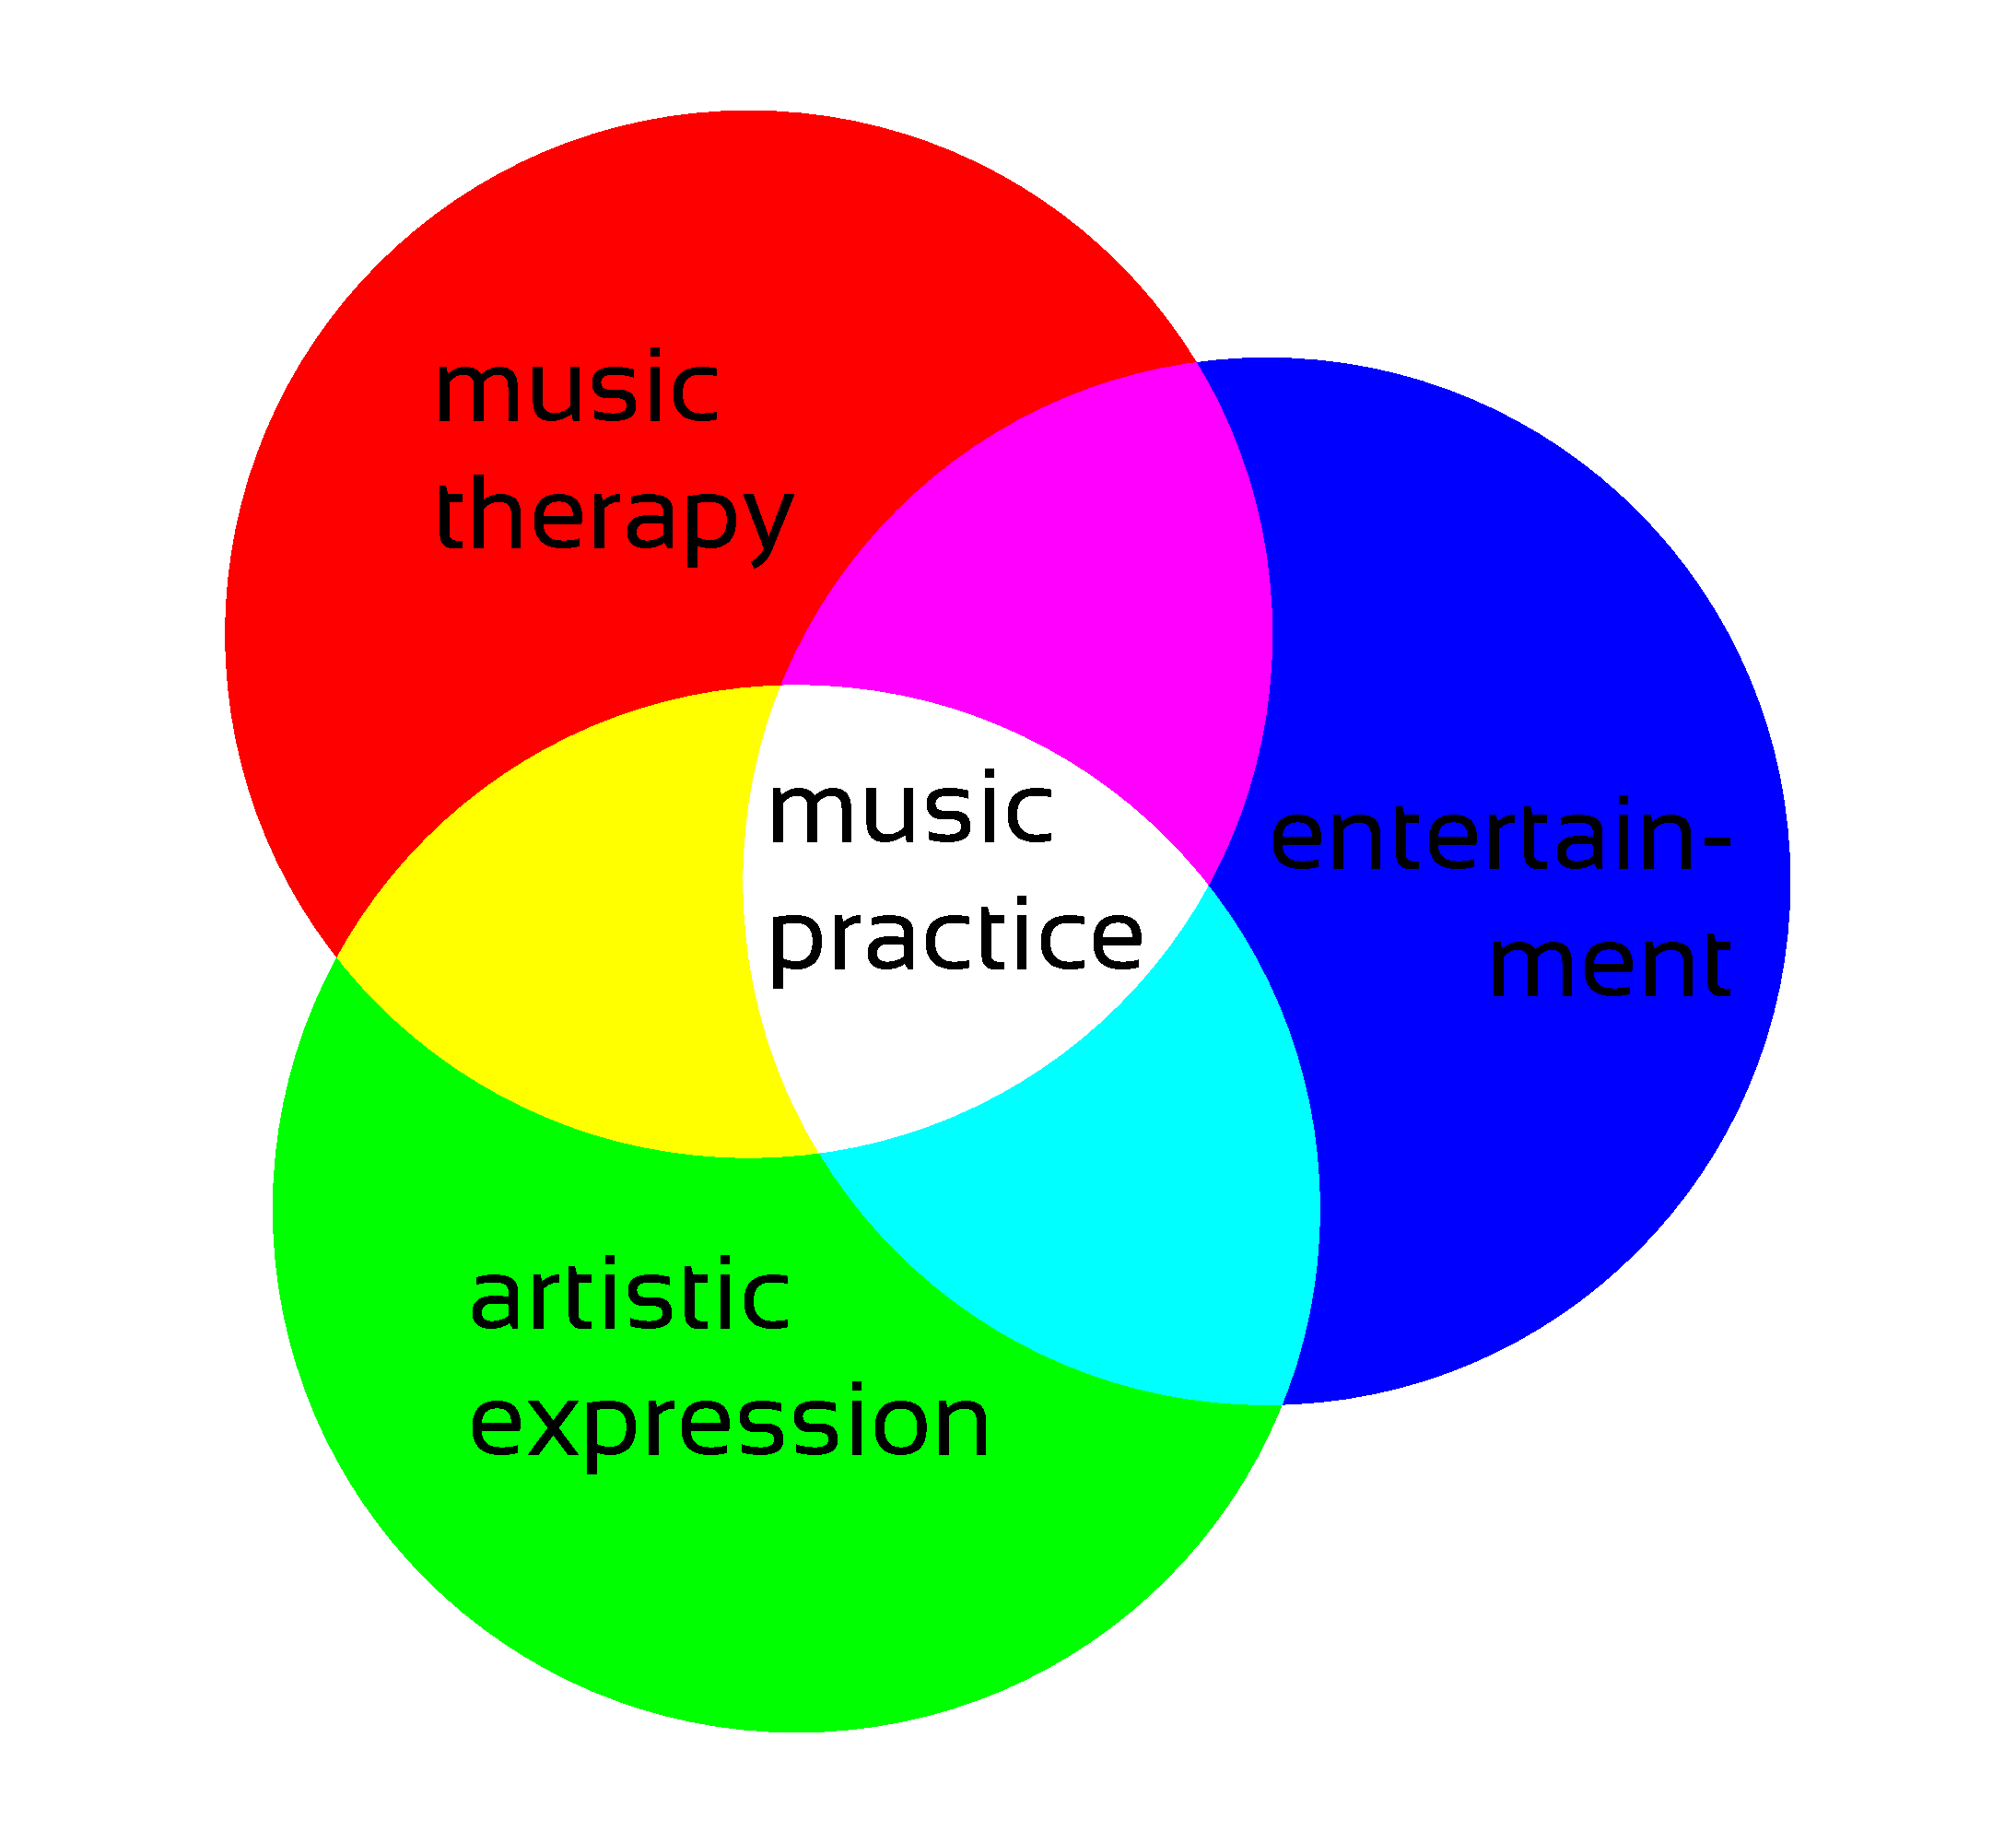
\includegraphics[width=\columnwidth]{media/musicThreefold-2.pdf}
	\caption{Considering artistic expression as a true purpose of musical practice unfolds and supports the span of meaning in music practice of people with special needs.}
	\label{fig:media_musicThreefold}
\end{figure}

We hope that the integration of target group members into the design cycle encourages a bilateral learning process.
An intense and fruitful experience for the participants is complemented by the circumstance that the involved researchers are able to identify challenges that are specific to this group, yet also reveal new perspectives on their respective research area.

In the next section, we will outline the research hypothesis and thereof arising questions. 
This is followed by a section giving a short overview on used research methods. 
The subsequent section tells about the state of the project to date and reports on the ongoing development in the involved research areas.
This is followed by a short description of the first field trip and it's initial results.
The paper concludes with a section on first insights and an outlook on further development.

\section{Research hypothesis}
\label{sec:research_objectives}

% some words about the research objective

The central hypothesis that this project examines can be broken down to the following sentence: 
\emph{Making the field of electronic music practice accessible to ND people empowers them to actively participate in an area that, after Headlam \cite{headlam2006-lea}, already paralleled specifics of ND thinking.}
Out of this hypothesis, four questions arise that we want to answer over the course of the project:

\begin{enumerate}
	\item Which aspects of electronic music are sufficiently interesting for the target group?
	\item In which sense does the active engagement with electronic music affect the aesthetic perception of target group members?
	\item In which direction do people of the target group develop their skills in electronic music making over the course of the project?
	\item What can we learn from people with autistic spectrum disorders when it comes to non-verbal communi- cation, creativity and music practice?
\end{enumerate}

\section{Implementation and research methods}
\label{sec:timeline}

%Here, we talk about the members of the group and which skills they contribute.
%Also, the design cycle is introduced and explained.

We investigate the above-mentioned research questions through three work packages (see also  Figure~\ref{fig:Designcycle}).

The first work package (WP1) is dedicated to investigative field work with target group members and the collection of data.
Interactive participatory design sessions are conducted in which the participants are introduced to contemporary electronic music and (later on) to instrument prototypes. 
A particular focus lies on open engagement with said instruments, providing an opportunity to explore and express.
During these sessions, the musical play is recorded and various other research material such as drawings, written comments and interviews of all involved people are collected.

In the second work package (WP2) the focus is set on data evaluation, coding and theory building.
The material gathered in WP1 is analysed and put into a broader context by incorporating knowledge gained from background research.
This will eventually lead towards a theory of electronic music practice for ND people.

WP3, the third work package, deals with \emph{conceptual synthesis} and instrument development; it aims to turn observations and derived theory made in WP1 and WP2 into practice by (a) rethinking the made theoretical considerations as practical guidelines and (b) creating instrument prototypes that are again used for the field work of WP1.

\begin{figure}
	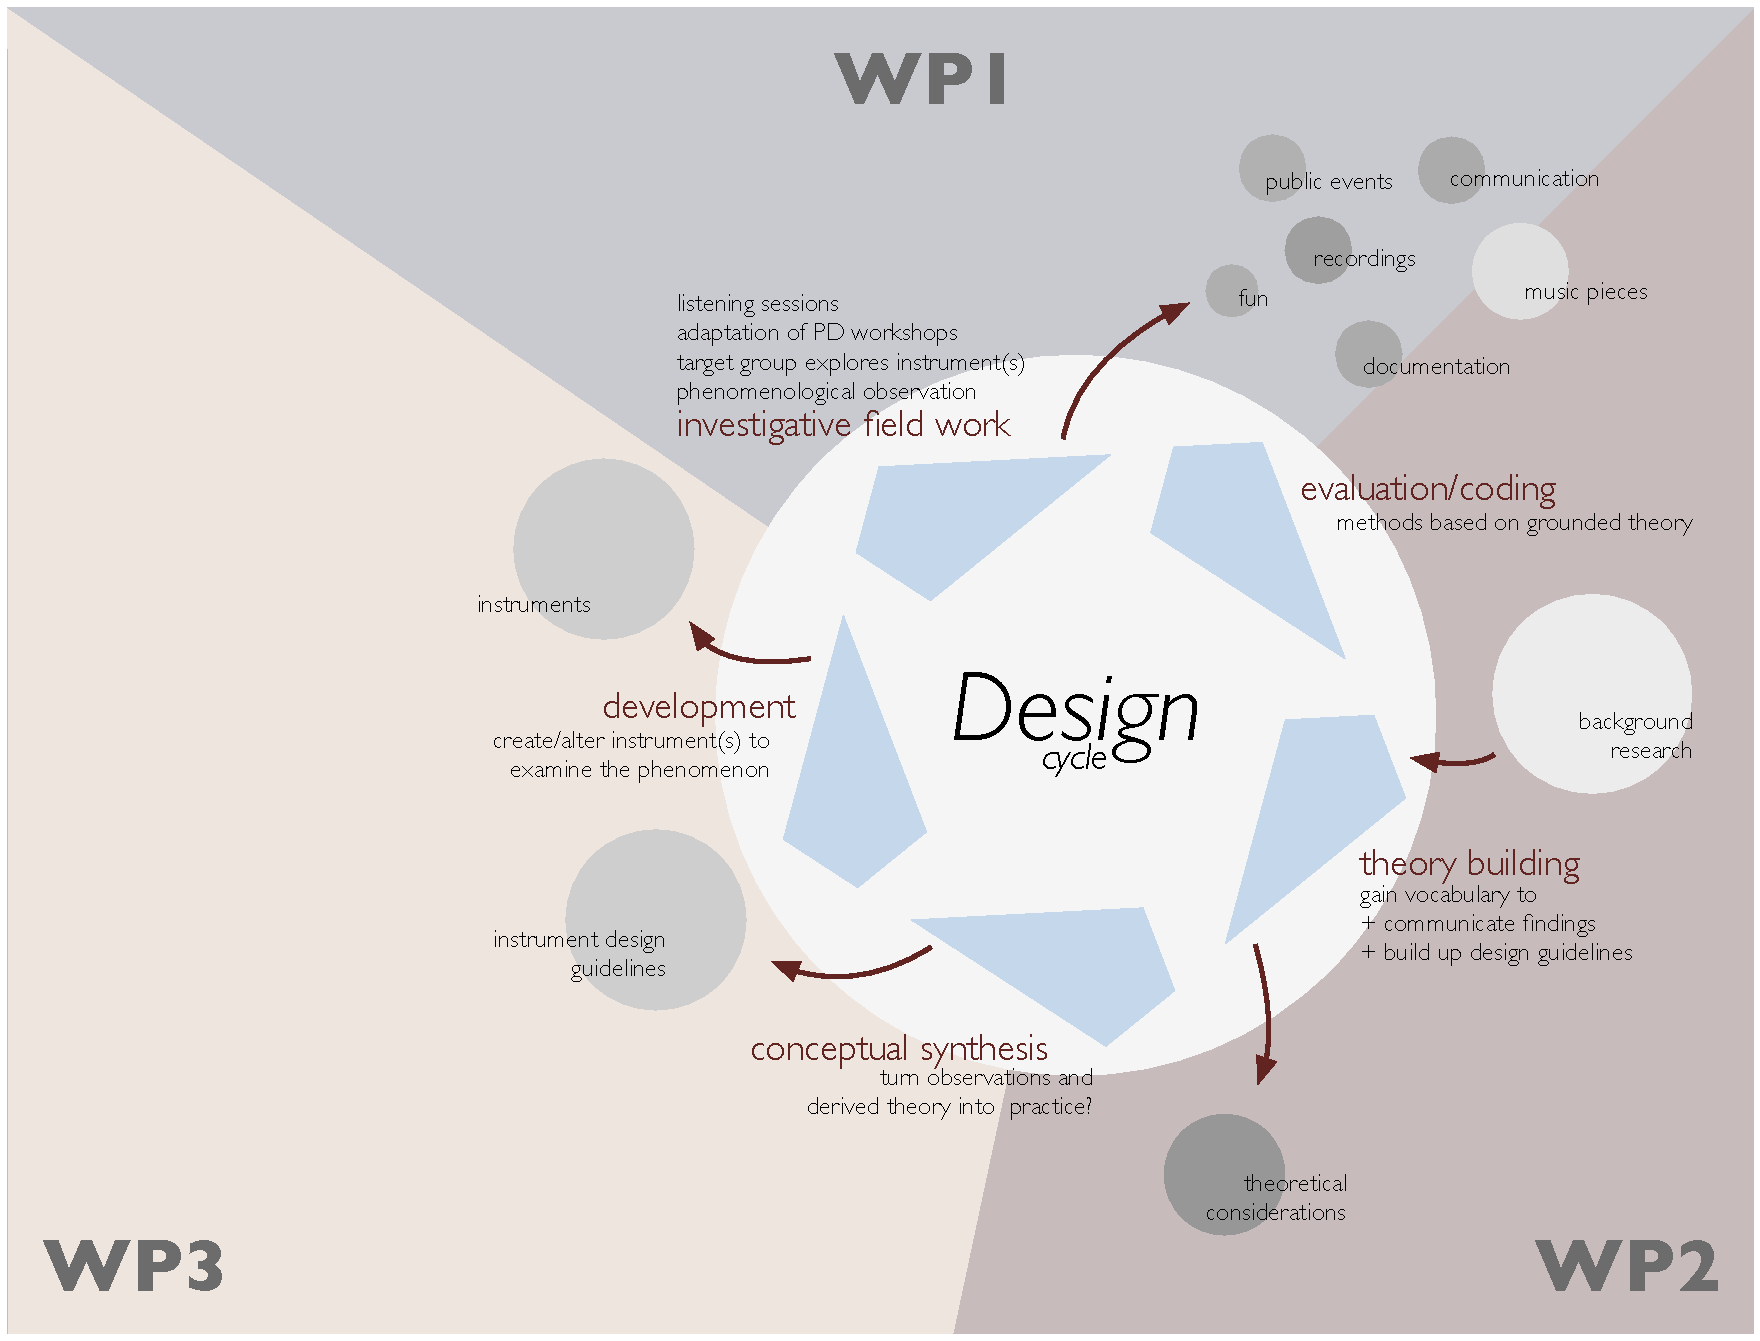
\includegraphics[width=\columnwidth]{media/DEINDDesignCycle.pdf}
	\caption{A structural overview of the design cycle showing interrelations of the WPs.}
	\label{fig:Designcycle}
\end{figure}

This project is mainly based on practice-oriented qualitative research methods~\cite{travers2001-qua}.
We extensively draw from participatory design and ethnomethodological research methods adapted to the target groups’ intrinsic character~\cite{schuler1993-par,strauss1990-bas}.
To fulfil the above-listed objectives, we apply a combination of experimental and theoretical methods that are based on both artistic and scientific research practices. 
These include 
(a) phenomenological observations of target group members exploring musical possibilities of instruments resulting in interviews, field notes and quantitative measurements, 
(b) grounded theory and phenomenological analysis based on recorded research material combined with background research in related fields and
(c) rapid software and hardware prototyping.
By their combination, new knowledge for specific electronic instruments are gained, generalised and finally fed back into the respective research areas.

The next section gives an overview on the ongoing research incorporating mentioned research methods.

\section{DEIND – A work in progress}
\label{sec:progress}

At the current state, the project made almost a full cycle in the design cycle.
It started with a kick-off meeting with all contributing members, followed  by a day trip to Nuorten Ystävät's supervised living center \emph{VillaKarelia} in Imatra, Finland where our target group members reside.
In the following workshop day, we discussed arising challenges and possible ideas for the system design which were eventually sorted and selected for the subsequent instrument prototyping. 

After finishing the prototypes, a five-day field trip to VillaKarelia was undertaken. 
Its main purpose was to take part in the daily routines of the target group members.
Initial ideas on where digital music practice could be fit into the highly structured days emerged during the stay, resulting in first sessions with interactive ambient soundscapes.
To date, the documentation material is partially analysed and will be reported in more detail in the short presentation. 

% TODO Also quite important is that we actually wanted to keep the fun factor in the equation: it should not be difficult, no heavy learning process should be involved. Why? Because the goal of the project is music practice not music therapy or learning.

% TODO observation: The people there are different. Different in the sense that they value other things than I expect from someone on the street.
% TODO tell which challenges arose out of the observations made
% TODO give examples for the prototype ideas and why they were considered
% TODO give detailed example on interactive soundscapes and tell that they were embedded in listening sessions

\subsection{Instrument prototyping}
\label{sec:instrument_prototyping}

We decided to develop two of the many ideas further, namely he rhythmical interaction part and the idea on room modes.

\subsubsection{Audio prototyping}
\label{sec:audio_prototyping}

Reports on the two to seventeen audio prototypes we did: 
the ambient system (complexRes), the FM matrix, the autoLoopPointer, the diodeRing, the noiseRing


\subsubsection{Sensor prototyping}
\label{sec:sensor_prototyping}
reports on the different sensors we looked at, e.g. switchDesigns (floor plan, imatra map)


\subsubsection{Interface prototyping}
\label{sec:interface_prototyping}

Mentions (again) that we're focusing mainly on textile-based interfaces.
Why is that so? 
	We have some knowledge and want to extent it. 
	Because textiles are nice to touch, give a lot of haptic feedback and are easily accepted (when showing the prototypes to people, they immediately grasp for them and hug them. Happened for real!)
We did an initial interface design with \emph{conductive fur}. 
We describe conductive fur, how we anticipated its usage, how it feels and how it works.
We as well give sound examples on how it sounds with and without added effects.

\subsubsection{Sonic environments}
\label{sec:sonic_environments}

Contact microphone attached to the ventilation outlet to capture its vibrations.
FM synthesis

\subsection{Field trip}
\label{sec:field_trip}










\subsection{Data analysis and first insights}
\label{sec:data_analysis}

This is a work in progress paper, more detailed information on the data analysis will be given in the short talk/poster.
First 

Describes what can be observed in the video session with participant 1 (rhythmical patterns).
Look at notes made in Imatra and report those as general observations.


oh my. so many lessons learned.
e.g. slowness, security, etc.



\section{Conclusion and Outlook}
\label{sec:outlook}

This paper outlined the DEIND project in which research on electronic music practice for neurodiverse people is conducted.
After a motivation for this work and an overview on the work done so far, initial insights were presented.
Based on these insights, we plan to continue this project and develop an interactive performance system that is closely adapted to target group's environment and their specific needs.

%ACKNOWLEDGMENTS are optional
\section{Acknowledgments}
The DEIND project on designing electronic instruments for \emph{ND} people is partially funded by the Aalto Media Factory of Aalto University, Helsinki.  


~\nocite{cappelen2012-mus,herstad2012-wha,herstad2012-mak,green2011agility,kleimola2011-vec,kleimola2010-fee,parker2011-a-s,parker2010-mod,valimaki2010-par,straus2011-ext,hegarty2006-noi,gurevich2007expression,burrows2010choreographer,bown2009understanding,jaarsma2012autism,hammel2011teaching,fard2012-wit,baggs2007-in,sinclair1993-don,wishart1994-aud,headlam2006-lea,2006-sou,campo2009-microsound,campo2009-the,m.-baalman2009-the,campo2008-objMod,wcd2011-scbook}


\bibliographystyle{abbrv}
\bibliography{/Users/tboverma/Public/unpub/BibTeX/bovermann} 

\end{multicols}

\end{document}